\textit{Nous avons fait le choix de débuter notre travail en rédigeant un cahier des charges sommaire. Ce premier travail, réalisé en équipe, nous a permis de cerner le sujet et de lister les besoins ainsi que les contraintes imposées. Le modèle de données proposé sera également exposé.}

\section{Fonctions principales}
		\subsubsection{Fournir des renseignements d'un schéma de BDD}
			\paragraph{tables}
				\begin{itemize}
					\item NAME
				\end{itemize}
			\paragraph{attributs}
				\begin{itemize}
					\item NAME
					\item TYPE
				\end{itemize}
			\paragraph{contraintes}
				\begin{itemize}
					\item PK
					\item FK
					\item UNIQUE
			  	\item CHECK + CHECK\_CLAUSE
				\end{itemize} 
		\subsubsection{Visualisation graphique}

\section{Fonctions contraintes}
	\subsection{Compatibilité \& extensibilité}
	L'outil développé devra être compatible avec les SGBDR les plus populaires (\emph{Mysql}, \emph{Postgresql}, \emph{Oracle}, etc.). L'architecture de l'application devra être pensée de manière à pouvoir étendre facilement la compatibilité avec de nouveaux SGBDR en utilisant, par exmple, des fichiers de configuration.
	\subsection{Utilisation d'Hibernate}
	L'objectif de ce projet étant l'application des outils vus pendant les cours de l'UE Gestion de données distribuées (GMIN210), l'outil développé devra utiliser l'ORM \emph{Hibernate} (librairie Java de mapping Object-Relationnel). Cette contrainte est imposée par le sujet.
	\subsection{Lecture des Métadonnées}
	Les métadonnées devront être chargées directement à partir des vues proposées par les différents SGBDR, via un connecteur. L'ORM \emph{Hibernate} étant imposé, le connecteur utilisé sera probablement \emph{JDBC}.

\section{Modélisation proposée}
\label{section:modelisation_proposee}

La figure~\ref{figure:diag_classe_fournit} présente le modèle de donnée de l'application, décrit dans le sujet. Il présente les éléments qui composent une base de données.

\begin{figure}[H]
\centering
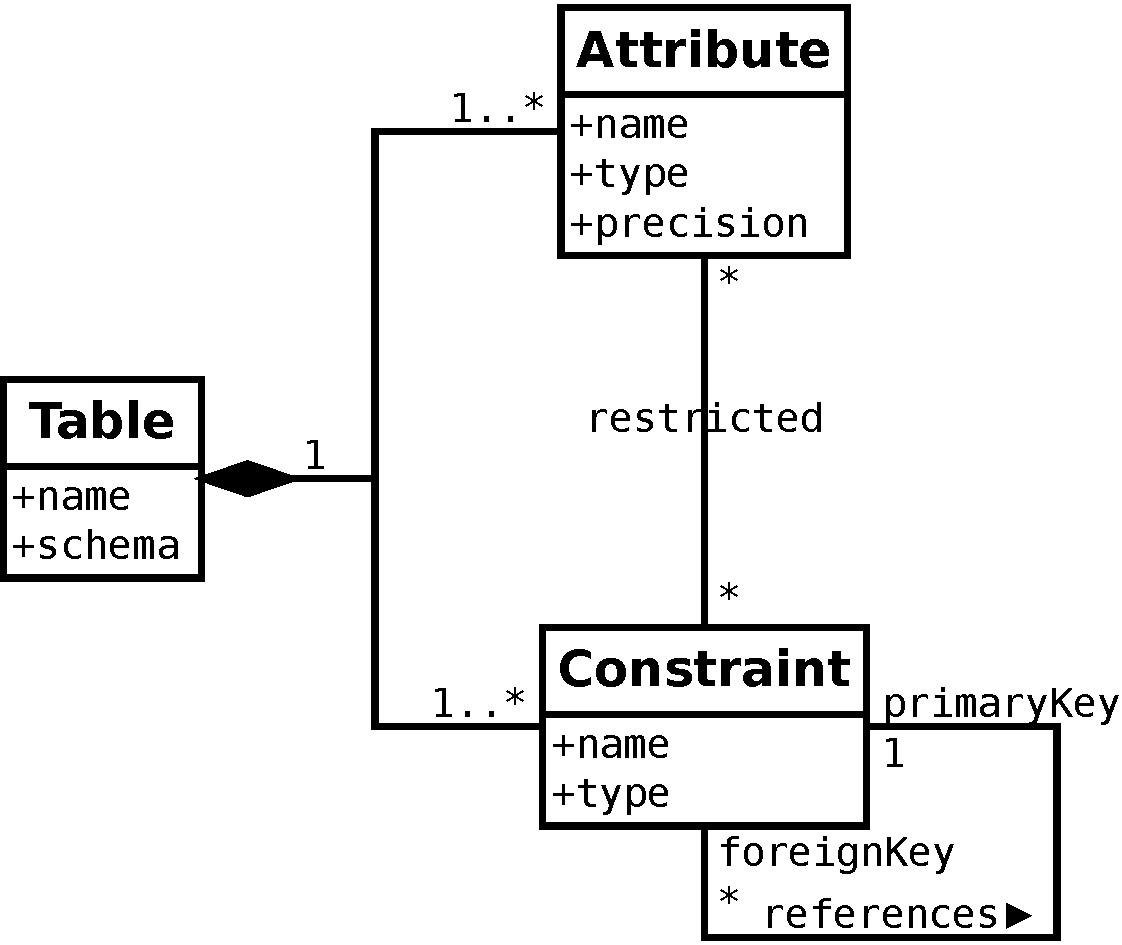
\includegraphics[width=0.6\textwidth]{files/diag_class_origine}
\caption{Diagramme de classe fournit.}
\label{figure:diag_classe_fournit}
\end{figure}

Une table est caractérisée par son nom et le nom du schéma dans lequel elle appartient. Elle est composée d'attributs et de contraintes. Un attribut, appartenant à une table, est caractérisé par son nom et son type (avec une précision). Une contrainte possède un nom et un type. Elle peut s'appliquer (restreindre) à un attribut et, dans le cas d'une clé étrangère, référencer une contrainte de clé primaire.